\documentclass[1p]{elsarticle_modified}
%\bibliographystyle{elsarticle-num}

%\usepackage[colorlinks]{hyperref}
%\usepackage{abbrmath_seonhwa} %\Abb, \Ascr, \Acal ,\Abf, \Afrak
\usepackage{amsfonts}
\usepackage{amssymb}
\usepackage{amsmath}
\usepackage{amsthm}
\usepackage{scalefnt}
\usepackage{amsbsy}
\usepackage{kotex}
\usepackage{caption}
\usepackage{subfig}
\usepackage{color}
\usepackage{graphicx}
\usepackage{xcolor} %% white, black, red, green, blue, cyan, magenta, yellow
\usepackage{float}
\usepackage{setspace}
\usepackage{hyperref}

\usepackage{tikz}
\usetikzlibrary{arrows}

\usepackage{multirow}
\usepackage{array} % fixed length table
\usepackage{hhline}

%%%%%%%%%%%%%%%%%%%%%
\makeatletter
\renewcommand*\env@matrix[1][\arraystretch]{%
	\edef\arraystretch{#1}%
	\hskip -\arraycolsep
	\let\@ifnextchar\new@ifnextchar
	\array{*\c@MaxMatrixCols c}}
\makeatother %https://tex.stackexchange.com/questions/14071/how-can-i-increase-the-line-spacing-in-a-matrix
%%%%%%%%%%%%%%%

\usepackage[normalem]{ulem}

\newcommand{\msout}[1]{\ifmmode\text{\sout{\ensuremath{#1}}}\else\sout{#1}\fi}
%SOURCE: \msout is \stkout macro in https://tex.stackexchange.com/questions/20609/strikeout-in-math-mode

\newcommand{\cancel}[1]{
	\ifmmode
	{\color{red}\msout{#1}}
	\else
	{\color{red}\sout{#1}}
	\fi
}

\newcommand{\add}[1]{
	{\color{blue}\uwave{#1}}
}

\newcommand{\replace}[2]{
	\ifmmode
	{\color{red}\msout{#1}}{\color{blue}\uwave{#2}}
	\else
	{\color{red}\sout{#1}}{\color{blue}\uwave{#2}}
	\fi
}

\newcommand{\Sol}{\mathcal{S}} %segment
\newcommand{\D}{D} %diagram
\newcommand{\A}{\mathcal{A}} %arc


%%%%%%%%%%%%%%%%%%%%%%%%%%%%%5 test

\def\sl{\operatorname{\textup{SL}}(2,\Cbb)}
\def\psl{\operatorname{\textup{PSL}}(2,\Cbb)}
\def\quan{\mkern 1mu \triangleright \mkern 1mu}

\theoremstyle{definition}
\newtheorem{thm}{Theorem}[section]
\newtheorem{prop}[thm]{Proposition}
\newtheorem{lem}[thm]{Lemma}
\newtheorem{ques}[thm]{Question}
\newtheorem{cor}[thm]{Corollary}
\newtheorem{defn}[thm]{Definition}
\newtheorem{exam}[thm]{Example}
\newtheorem{rmk}[thm]{Remark}
\newtheorem{alg}[thm]{Algorithm}

\newcommand{\I}{\sqrt{-1}}
\begin{document}

%\begin{frontmatter}
%
%\title{Boundary parabolic representations of knots up to 8 crossings}
%
%%% Group authors per affiliation:
%\author{Yunhi Cho} 
%\address{Department of Mathematics, University of Seoul, Seoul, Korea}
%\ead{yhcho@uos.ac.kr}
%
%
%\author{Seonhwa Kim} %\fnref{s_kim}}
%\address{Center for Geometry and Physics, Institute for Basic Science, Pohang, 37673, Korea}
%\ead{ryeona17@ibs.re.kr}
%
%\author{Hyuk Kim}
%\address{Department of Mathematical Sciences, Seoul National University, Seoul 08826, Korea}
%\ead{hyukkim@snu.ac.kr}
%
%\author{Seokbeom Yoon}
%\address{Department of Mathematical Sciences, Seoul National University, Seoul, 08826,  Korea}
%\ead{sbyoon15@snu.ac.kr}
%
%\begin{abstract}
%We find all boundary parabolic representation of knots up to 8 crossings.
%
%\end{abstract}
%\begin{keyword}
%    \MSC[2010] 57M25 
%\end{keyword}
%
%\end{frontmatter}

%\linenumbers
%\tableofcontents
%
\newcommand\colored[1]{\textcolor{white}{\rule[-0.35ex]{0.8em}{1.4ex}}\kern-0.8em\color{red} #1}%
%\newcommand\colored[1]{\textcolor{white}{ #1}\kern-2.17ex	\textcolor{white}{ #1}\kern-1.81ex	\textcolor{white}{ #1}\kern-2.15ex\color{red}#1	}

{\Large $\underline{12n_{0264}~(K12n_{0264})}$}

\setlength{\tabcolsep}{10pt}
\renewcommand{\arraystretch}{1.6}
\vspace{1cm}\begin{tabular}{m{100pt}>{\centering\arraybackslash}m{274pt}}
\multirow{5}{120pt}{
	\centering
	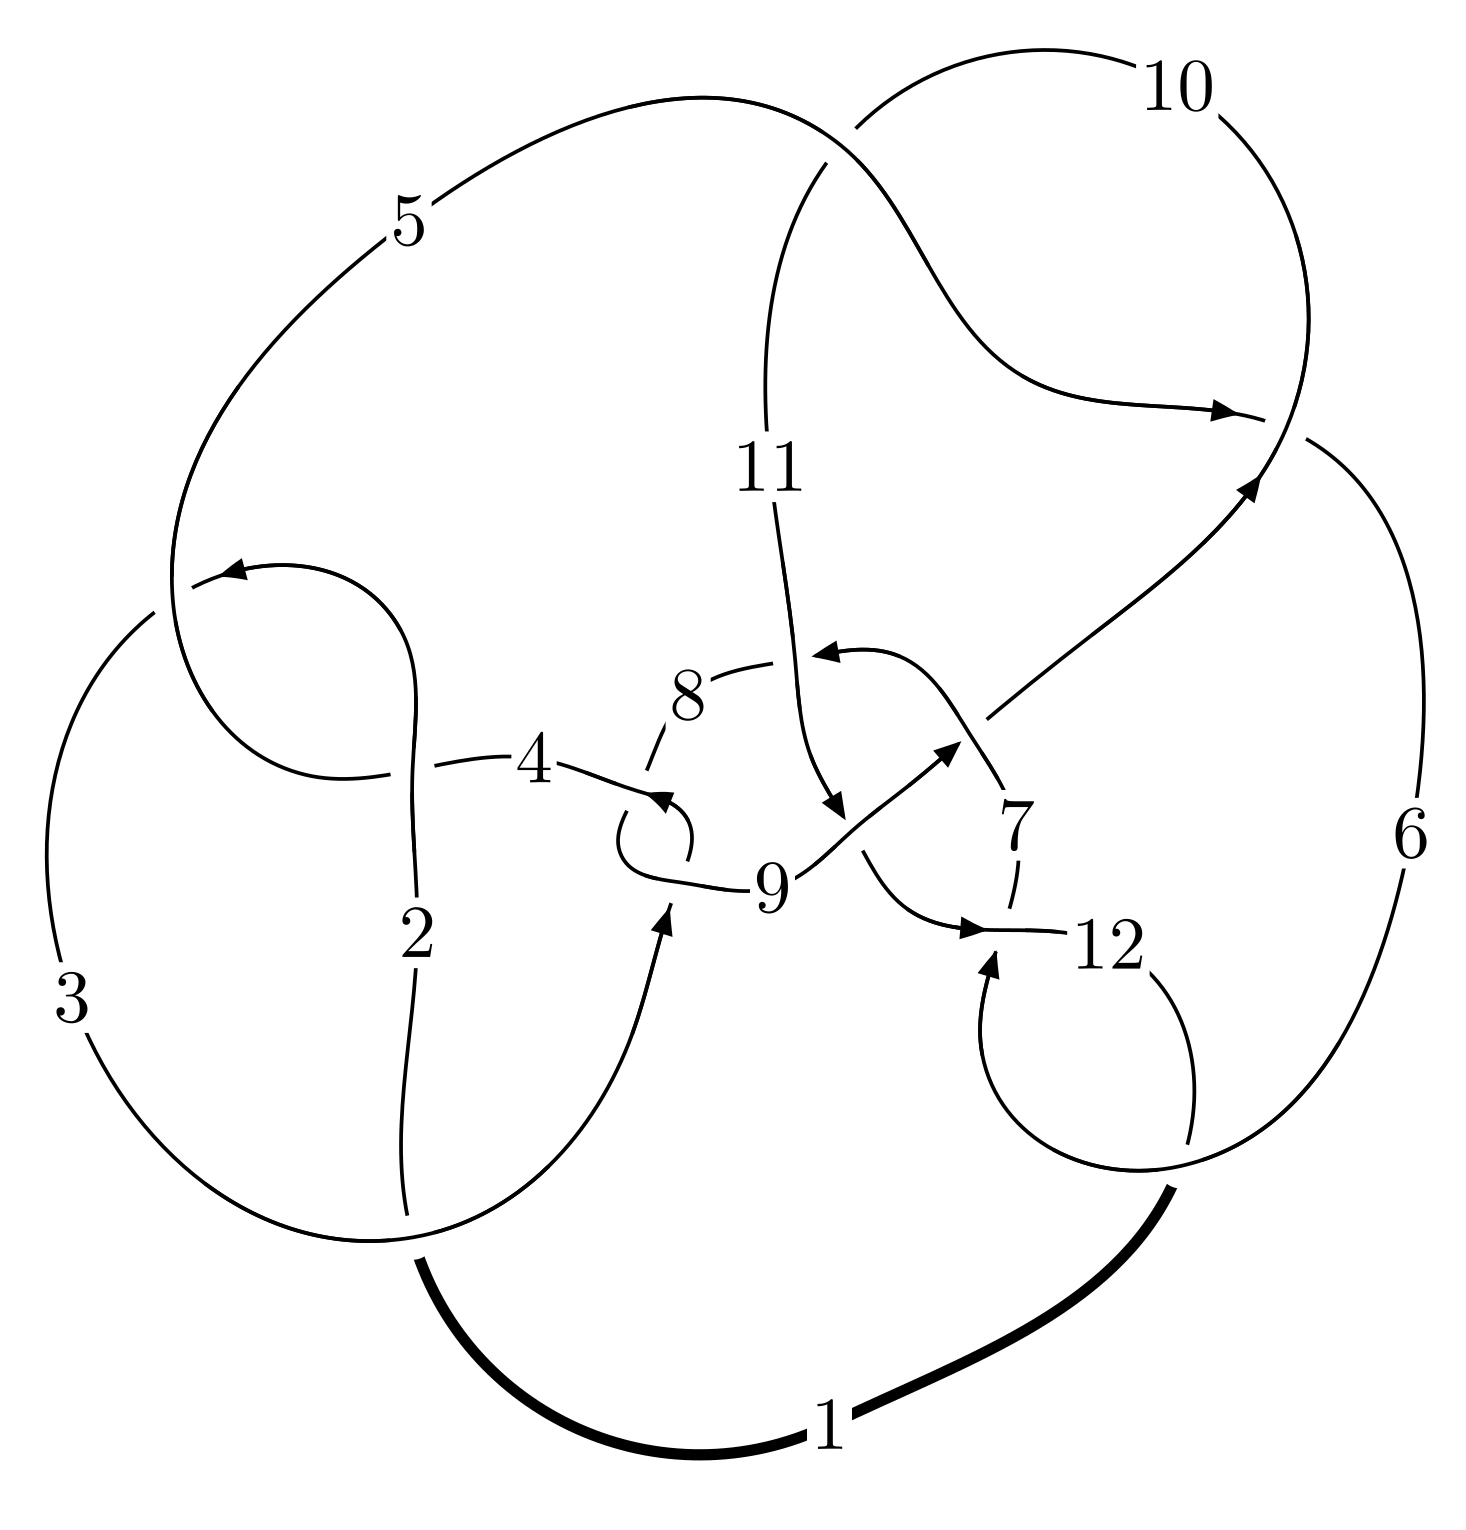
\includegraphics[width=112pt]{../../../GIT/diagram.site/Diagrams/png/2353_12n_0264.png}\\
\ \ \ A knot diagram\footnotemark}&
\allowdisplaybreaks
\textbf{Linearized knot diagam} \\
\cline{2-2}
 &
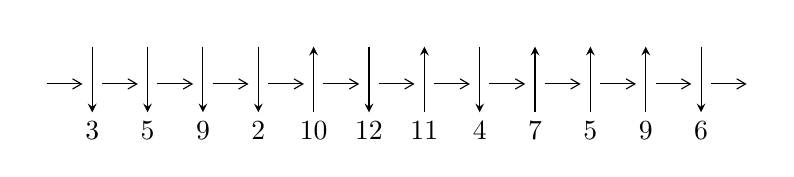
\begin{tikzpicture}[x=20pt, y=17pt]
	% nodes
	\node (C0) at (0, 0) {};
	\node (C1) at (1, 0) {};
	\node (C1U) at (1, +1) {};
	\node (C1D) at (1, -1) {3};

	\node (C2) at (2, 0) {};
	\node (C2U) at (2, +1) {};
	\node (C2D) at (2, -1) {5};

	\node (C3) at (3, 0) {};
	\node (C3U) at (3, +1) {};
	\node (C3D) at (3, -1) {9};

	\node (C4) at (4, 0) {};
	\node (C4U) at (4, +1) {};
	\node (C4D) at (4, -1) {2};

	\node (C5) at (5, 0) {};
	\node (C5U) at (5, +1) {};
	\node (C5D) at (5, -1) {10};

	\node (C6) at (6, 0) {};
	\node (C6U) at (6, +1) {};
	\node (C6D) at (6, -1) {12};

	\node (C7) at (7, 0) {};
	\node (C7U) at (7, +1) {};
	\node (C7D) at (7, -1) {11};

	\node (C8) at (8, 0) {};
	\node (C8U) at (8, +1) {};
	\node (C8D) at (8, -1) {4};

	\node (C9) at (9, 0) {};
	\node (C9U) at (9, +1) {};
	\node (C9D) at (9, -1) {7};

	\node (C10) at (10, 0) {};
	\node (C10U) at (10, +1) {};
	\node (C10D) at (10, -1) {5};

	\node (C11) at (11, 0) {};
	\node (C11U) at (11, +1) {};
	\node (C11D) at (11, -1) {9};

	\node (C12) at (12, 0) {};
	\node (C12U) at (12, +1) {};
	\node (C12D) at (12, -1) {6};
	\node (C13) at (13, 0) {};

	% arrows
	\draw[->,>={angle 60}]
	(C0) edge (C1) (C1) edge (C2) (C2) edge (C3) (C3) edge (C4) (C4) edge (C5) (C5) edge (C6) (C6) edge (C7) (C7) edge (C8) (C8) edge (C9) (C9) edge (C10) (C10) edge (C11) (C11) edge (C12) (C12) edge (C13) ;	\draw[->,>=stealth]
	(C1U) edge (C1D) (C2U) edge (C2D) (C3U) edge (C3D) (C4U) edge (C4D) (C5D) edge (C5U) (C6U) edge (C6D) (C7D) edge (C7U) (C8U) edge (C8D) (C9D) edge (C9U) (C10D) edge (C10U) (C11D) edge (C11U) (C12U) edge (C12D) ;
	\end{tikzpicture} \\
\hhline{~~} \\& 
\textbf{Solving Sequence} \\ \cline{2-2} 
 &
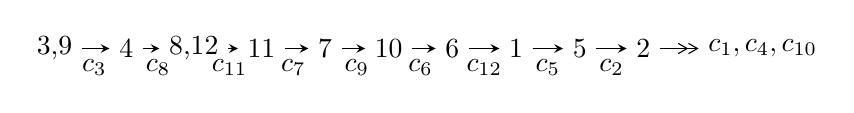
\begin{tikzpicture}[x=23pt, y=7pt]
	% node
	\node (A0) at (-1/8, 0) {3,9};
	\node (A1) at (1, 0) {4};
	\node (A2) at (33/16, 0) {8,12};
	\node (A3) at (25/8, 0) {11};
	\node (A4) at (33/8, 0) {7};
	\node (A5) at (41/8, 0) {10};
	\node (A6) at (49/8, 0) {6};
	\node (A7) at (57/8, 0) {1};
	\node (A8) at (65/8, 0) {5};
	\node (A9) at (73/8, 0) {2};
	\node (C1) at (1/2, -1) {$c_{3}$};
	\node (C2) at (3/2, -1) {$c_{8}$};
	\node (C3) at (21/8, -1) {$c_{11}$};
	\node (C4) at (29/8, -1) {$c_{7}$};
	\node (C5) at (37/8, -1) {$c_{9}$};
	\node (C6) at (45/8, -1) {$c_{6}$};
	\node (C7) at (53/8, -1) {$c_{12}$};
	\node (C8) at (61/8, -1) {$c_{5}$};
	\node (C9) at (69/8, -1) {$c_{2}$};
	\node (A10) at (11, 0) {$c_{1},c_{4},c_{10}$};

	% edge
	\draw[->,>=stealth]	
	(A0) edge (A1) (A1) edge (A2) (A2) edge (A3) (A3) edge (A4) (A4) edge (A5) (A5) edge (A6) (A6) edge (A7) (A7) edge (A8) (A8) edge (A9) ;
	\draw[->>,>={angle 60}]	
	(A9) edge (A10);
\end{tikzpicture} \\ 

\end{tabular} \\

\footnotetext{
The image of knot diagram is generated by the software ``\textbf{Draw programme}" developed by Andrew Bartholomew(\url{http://www.layer8.co.uk/maths/draw/index.htm\#Running-draw}), where we modified some parts for our purpose(\url{https://github.com/CATsTAILs/LinksPainter}).
}\phantom \\ \newline 
\centering \textbf{Ideals for irreducible components\footnotemark of $X_{\text{par}}$} 
 
\begin{align*}
I^u_{1}&=\langle 
3.93403\times10^{149} u^{37}-1.74178\times10^{149} u^{36}+\cdots+2.21546\times10^{152} b+1.76661\times10^{154},\\
\phantom{I^u_{1}}&\phantom{= \langle  }7.93734\times10^{149} u^{37}-3.29411\times10^{149} u^{36}+\cdots+4.43092\times10^{152} a+3.55362\times10^{154},\\
\phantom{I^u_{1}}&\phantom{= \langle  }u^{38}- u^{37}+\cdots+86016 u-25088\rangle \\
I^u_{2}&=\langle 
8082115793 u^{16}+864266486 u^{15}+\cdots+5782655035 b-29654101499,\\
\phantom{I^u_{2}}&\phantom{= \langle  }682951511 u^{16}-479427583 u^{15}+\cdots+5782655035 a-12663191293,\;u^{17}+6 u^{15}+\cdots-3 u+1\rangle \\
\\
I^v_{1}&=\langle 
a,\;-579074 v^8+1101995 v^7+\cdots+5353327 b+7952402,\\
\phantom{I^v_{1}}&\phantom{= \langle  }v^9- v^8-8 v^7+v^6+33 v^5+23 v^4-14 v^3-2 v^2+3 v-7\rangle \\
\end{align*}
\raggedright * 3 irreducible components of $\dim_{\mathbb{C}}=0$, with total 64 representations.\\
\footnotetext{All coefficients of polynomials are rational numbers. But the coefficients are sometimes approximated in decimal forms when there is not enough margin.}
\newpage
\renewcommand{\arraystretch}{1}
\centering \section*{I. $I^u_{1}= \langle 3.93\times10^{149} u^{37}-1.74\times10^{149} u^{36}+\cdots+2.22\times10^{152} b+1.77\times10^{154},\;7.94\times10^{149} u^{37}-3.29\times10^{149} u^{36}+\cdots+4.43\times10^{152} a+3.55\times10^{154},\;u^{38}- u^{37}+\cdots+86016 u-25088 \rangle$}
\flushleft \textbf{(i) Arc colorings}\\
\begin{tabular}{m{7pt} m{180pt} m{7pt} m{180pt} }
\flushright $a_{3}=$&$\begin{pmatrix}1\\0\end{pmatrix}$ \\
\flushright $a_{9}=$&$\begin{pmatrix}0\\u\end{pmatrix}$ \\
\flushright $a_{4}=$&$\begin{pmatrix}1\\u^2\end{pmatrix}$ \\
\flushright $a_{8}=$&$\begin{pmatrix}u\\u^3+u\end{pmatrix}$ \\
\flushright $a_{12}=$&$\begin{pmatrix}-0.00179135 u^{37}+0.000743437 u^{36}+\cdots+147.911 u-80.2006\\-0.00177572 u^{37}+0.000786192 u^{36}+\cdots+151.635 u-79.7401\end{pmatrix}$ \\
\flushright $a_{11}=$&$\begin{pmatrix}-0.00179135 u^{37}+0.000743437 u^{36}+\cdots+147.911 u-80.2006\\-0.00247624 u^{37}+0.00101022 u^{36}+\cdots+196.831 u-106.030\end{pmatrix}$ \\
\flushright $a_{7}=$&$\begin{pmatrix}-0.00108938 u^{37}+0.000479390 u^{36}+\cdots+86.4568 u-38.9386\\-0.00129295 u^{37}+0.000455453 u^{36}+\cdots+89.7492 u-44.1198\end{pmatrix}$ \\
\flushright $a_{10}=$&$\begin{pmatrix}-0.00134130 u^{37}+0.000498496 u^{36}+\cdots+100.346 u-57.3777\\-0.00207949 u^{37}+0.000840213 u^{36}+\cdots+166.563 u-92.5692\end{pmatrix}$ \\
\flushright $a_{6}=$&$\begin{pmatrix}-0.00126938 u^{37}+0.000412248 u^{36}+\cdots+85.1965 u-49.2329\\-0.00261068 u^{37}+0.000910744 u^{36}+\cdots+185.542 u-106.611\end{pmatrix}$ \\
\flushright $a_{1}=$&$\begin{pmatrix}-0.000219442 u^{37}+0.000183073 u^{36}+\cdots+30.0161 u-10.6041\\-0.000132258 u^{37}+0.000107784 u^{36}+\cdots+18.7525 u-7.96288\end{pmatrix}$ \\
\flushright $a_{5}=$&$\begin{pmatrix}0.0000871841 u^{37}-0.0000752884 u^{36}+\cdots-11.2636 u+2.64124\\-0.000143931 u^{37}+0.000121946 u^{36}+\cdots+19.9165 u-7.66444\end{pmatrix}$ \\
\flushright $a_{2}=$&$\begin{pmatrix}-0.0000871841 u^{37}+0.0000752884 u^{36}+\cdots+11.2636 u-2.64124\\-0.000132258 u^{37}+0.000107784 u^{36}+\cdots+18.7525 u-7.96288\end{pmatrix}$\\&\end{tabular}
\flushleft \textbf{(ii) Obstruction class $= -1$}\\~\\
\flushleft \textbf{(iii) Cusp Shapes $= 0.00823228 u^{37}-0.00319378 u^{36}+\cdots-645.161 u+373.502$}\\~\\
\newpage\renewcommand{\arraystretch}{1}
\flushleft \textbf{(iv) u-Polynomials at the component}\newline \\
\begin{tabular}{m{50pt}|m{274pt}}
Crossings & \hspace{64pt}u-Polynomials at each crossing \\
\hline $$\begin{aligned}c_{1}\end{aligned}$$&$\begin{aligned}
&u^{38}+46 u^{36}+\cdots+6958 u+2401
\end{aligned}$\\
\hline $$\begin{aligned}c_{2},c_{4}\end{aligned}$$&$\begin{aligned}
&u^{38}-16 u^{37}+\cdots+378 u-49
\end{aligned}$\\
\hline $$\begin{aligned}c_{3},c_{8}\end{aligned}$$&$\begin{aligned}
&u^{38}- u^{37}+\cdots+86016 u-25088
\end{aligned}$\\
\hline $$\begin{aligned}c_{5},c_{10}\end{aligned}$$&$\begin{aligned}
&u^{38}-2 u^{37}+\cdots-3904 u-5873
\end{aligned}$\\
\hline $$\begin{aligned}c_{6},c_{12}\end{aligned}$$&$\begin{aligned}
&u^{38}-3 u^{37}+\cdots-446 u+44
\end{aligned}$\\
\hline $$\begin{aligned}c_{7}\end{aligned}$$&$\begin{aligned}
&u^{38}+u^{37}+\cdots+40881797 u+3617129
\end{aligned}$\\
\hline $$\begin{aligned}c_{9}\end{aligned}$$&$\begin{aligned}
&u^{38}+4 u^{37}+\cdots-114 u-17
\end{aligned}$\\
\hline $$\begin{aligned}c_{11}\end{aligned}$$&$\begin{aligned}
&u^{38}+u^{37}+\cdots+79046 u-14009
\end{aligned}$\\
\hline
\end{tabular}\\~\\
\newpage\renewcommand{\arraystretch}{1}
\flushleft \textbf{(v) Riley Polynomials at the component}\newline \\
\begin{tabular}{m{50pt}|m{274pt}}
Crossings & \hspace{64pt}Riley Polynomials at each crossing \\
\hline $$\begin{aligned}c_{1}\end{aligned}$$&$\begin{aligned}
&y^{38}+92 y^{37}+\cdots+262856678 y+5764801
\end{aligned}$\\
\hline $$\begin{aligned}c_{2},c_{4}\end{aligned}$$&$\begin{aligned}
&y^{38}+46 y^{36}+\cdots-6958 y+2401
\end{aligned}$\\
\hline $$\begin{aligned}c_{3},c_{8}\end{aligned}$$&$\begin{aligned}
&y^{38}+69 y^{37}+\cdots+3750756352 y+629407744
\end{aligned}$\\
\hline $$\begin{aligned}c_{5},c_{10}\end{aligned}$$&$\begin{aligned}
&y^{38}-12 y^{37}+\cdots-781291844 y+34492129
\end{aligned}$\\
\hline $$\begin{aligned}c_{6},c_{12}\end{aligned}$$&$\begin{aligned}
&y^{38}+35 y^{37}+\cdots-111884 y+1936
\end{aligned}$\\
\hline $$\begin{aligned}c_{7}\end{aligned}$$&$\begin{aligned}
&y^{38}-107 y^{37}+\cdots-346184004395873 y+13083622202641
\end{aligned}$\\
\hline $$\begin{aligned}c_{9}\end{aligned}$$&$\begin{aligned}
&y^{38}-6 y^{37}+\cdots-8270 y+289
\end{aligned}$\\
\hline $$\begin{aligned}c_{11}\end{aligned}$$&$\begin{aligned}
&y^{38}-69 y^{37}+\cdots-9544952050 y+196252081
\end{aligned}$\\
\hline
\end{tabular}\\~\\
\newpage\flushleft \textbf{(vi) Complex Volumes and Cusp Shapes}
$$\begin{array}{c|c|c}  
\text{Solutions to }I^u_{1}& \I (\text{vol} + \sqrt{-1}CS) & \text{Cusp shape}\\
 \hline 
\begin{aligned}
u &= -0.542649 + 0.614305 I \\
a &= \phantom{-}0.515994 + 1.233570 I \\
b &= -0.104502 + 0.163985 I\end{aligned}
 & \phantom{-}1.68943 + 7.69679 I & -0.16453 - 13.04445 I \\ \hline\begin{aligned}
u &= -0.542649 - 0.614305 I \\
a &= \phantom{-}0.515994 - 1.233570 I \\
b &= -0.104502 - 0.163985 I\end{aligned}
 & \phantom{-}1.68943 - 7.69679 I & -0.16453 + 13.04445 I \\ \hline\begin{aligned}
u &= \phantom{-}0.072090 + 0.744709 I \\
a &= \phantom{-}0.81163 - 1.20274 I \\
b &= \phantom{-}0.230747 + 0.056669 I\end{aligned}
 & \phantom{-}3.31755 + 0.54950 I & \phantom{-}6.15791 + 2.31967 I \\ \hline\begin{aligned}
u &= \phantom{-}0.072090 - 0.744709 I \\
a &= \phantom{-}0.81163 + 1.20274 I \\
b &= \phantom{-}0.230747 - 0.056669 I\end{aligned}
 & \phantom{-}3.31755 - 0.54950 I & \phantom{-}6.15791 - 2.31967 I \\ \hline\begin{aligned}
u &= -0.554003 + 0.499646 I \\
a &= \phantom{-}0.259417 + 1.163440 I \\
b &= \phantom{-}0.126830 + 0.775649 I\end{aligned}
 & -1.38624 + 1.33481 I & -2.97345 - 3.66862 I \\ \hline\begin{aligned}
u &= -0.554003 - 0.499646 I \\
a &= \phantom{-}0.259417 - 1.163440 I \\
b &= \phantom{-}0.126830 - 0.775649 I\end{aligned}
 & -1.38624 - 1.33481 I & -2.97345 + 3.66862 I \\ \hline\begin{aligned}
u &= \phantom{-}0.434969 + 0.601443 I \\
a &= \phantom{-}1.185780 - 0.546611 I \\
b &= \phantom{-}0.144861 + 0.163719 I\end{aligned}
 & \phantom{-}1.48961 + 0.57943 I & \phantom{-}5.02569 - 0.39325 I \\ \hline\begin{aligned}
u &= \phantom{-}0.434969 - 0.601443 I \\
a &= \phantom{-}1.185780 + 0.546611 I \\
b &= \phantom{-}0.144861 - 0.163719 I\end{aligned}
 & \phantom{-}1.48961 - 0.57943 I & \phantom{-}5.02569 + 0.39325 I \\ \hline\begin{aligned}
u &= \phantom{-}0.606671 + 0.412287 I \\
a &= -1.202140 + 0.417819 I \\
b &= -1.72769 - 0.34007 I\end{aligned}
 & -4.47346 + 0.84284 I & -11.66035 - 0.97344 I \\ \hline\begin{aligned}
u &= \phantom{-}0.606671 - 0.412287 I \\
a &= -1.202140 - 0.417819 I \\
b &= -1.72769 + 0.34007 I\end{aligned}
 & -4.47346 - 0.84284 I & -11.66035 + 0.97344 I\\
 \hline 
 \end{array}$$\newpage$$\begin{array}{c|c|c}  
\text{Solutions to }I^u_{1}& \I (\text{vol} + \sqrt{-1}CS) & \text{Cusp shape}\\
 \hline 
\begin{aligned}
u &= \phantom{-}0.185752 + 1.318190 I \\
a &= \phantom{-}0.519872 + 0.356267 I \\
b &= -0.524833 + 0.069232 I\end{aligned}
 & -2.12322 - 4.24125 I & -4.26882 + 3.51292 I \\ \hline\begin{aligned}
u &= \phantom{-}0.185752 - 1.318190 I \\
a &= \phantom{-}0.519872 - 0.356267 I \\
b &= -0.524833 - 0.069232 I\end{aligned}
 & -2.12322 + 4.24125 I & -4.26882 - 3.51292 I \\ \hline\begin{aligned}
u &= \phantom{-}0.626028 + 0.000453 I \\
a &= \phantom{-}0.99835 + 1.48871 I \\
b &= \phantom{-}1.84598 + 1.42085 I\end{aligned}
 & \phantom{-}0.61462 + 3.26287 I & -1.84851 - 7.14359 I \\ \hline\begin{aligned}
u &= \phantom{-}0.626028 - 0.000453 I \\
a &= \phantom{-}0.99835 - 1.48871 I \\
b &= \phantom{-}1.84598 - 1.42085 I\end{aligned}
 & \phantom{-}0.61462 - 3.26287 I & -1.84851 + 7.14359 I \\ \hline\begin{aligned}
u &= \phantom{-}0.220678 + 0.522522 I \\
a &= -0.299614 - 0.840555 I \\
b &= -2.25916 - 0.15809 I\end{aligned}
 & -0.41969 - 2.46857 I & \phantom{-}5.02234 + 6.21524 I \\ \hline\begin{aligned}
u &= \phantom{-}0.220678 - 0.522522 I \\
a &= -0.299614 + 0.840555 I \\
b &= -2.25916 + 0.15809 I\end{aligned}
 & -0.41969 + 2.46857 I & \phantom{-}5.02234 - 6.21524 I \\ \hline\begin{aligned}
u &= \phantom{-}0.134435 + 0.540176 I \\
a &= \phantom{-}1.65614 + 0.96243 I \\
b &= \phantom{-}0.467042 + 0.770777 I\end{aligned}
 & \phantom{-}0.34862 + 2.64648 I & \phantom{-}0.38453 - 4.62015 I \\ \hline\begin{aligned}
u &= \phantom{-}0.134435 - 0.540176 I \\
a &= \phantom{-}1.65614 - 0.96243 I \\
b &= \phantom{-}0.467042 - 0.770777 I\end{aligned}
 & \phantom{-}0.34862 - 2.64648 I & \phantom{-}0.38453 + 4.62015 I \\ \hline\begin{aligned}
u &= -0.487313\phantom{ +0.000000I} \\
a &= -0.299932\phantom{ +0.000000I} \\
b &= -0.879403\phantom{ +0.000000I}\end{aligned}
 & -1.21395\phantom{ +0.000000I} & -9.56810\phantom{ +0.000000I} \\ \hline\begin{aligned}
u &= -1.68632 + 0.08026 I \\
a &= \phantom{-}0.014317 + 0.422528 I \\
b &= -0.16420 + 1.88746 I\end{aligned}
 & \phantom{-}1.94242 + 0.25898 I & \phantom{-0.000000 } 0\\
 \hline 
 \end{array}$$\newpage$$\begin{array}{c|c|c}  
\text{Solutions to }I^u_{1}& \I (\text{vol} + \sqrt{-1}CS) & \text{Cusp shape}\\
 \hline 
\begin{aligned}
u &= -1.68632 - 0.08026 I \\
a &= \phantom{-}0.014317 - 0.422528 I \\
b &= -0.16420 - 1.88746 I\end{aligned}
 & \phantom{-}1.94242 - 0.25898 I & \phantom{-0.000000 } 0 \\ \hline\begin{aligned}
u &= \phantom{-}1.86202\phantom{ +0.000000I} \\
a &= -0.669370\phantom{ +0.000000I} \\
b &= \phantom{-}1.04021\phantom{ +0.000000I}\end{aligned}
 & -6.81012\phantom{ +0.000000I} & \phantom{-0.000000 } 0 \\ \hline\begin{aligned}
u &= -0.78573 + 1.74324 I \\
a &= -1.105090 - 0.592834 I \\
b &= -0.214357 - 0.763758 I\end{aligned}
 & \phantom{-}6.33444 - 4.25779 I & \phantom{-0.000000 } 0 \\ \hline\begin{aligned}
u &= -0.78573 - 1.74324 I \\
a &= -1.105090 + 0.592834 I \\
b &= -0.214357 + 0.763758 I\end{aligned}
 & \phantom{-}6.33444 + 4.25779 I & \phantom{-0.000000 } 0 \\ \hline\begin{aligned}
u &= \phantom{-}0.36940 + 1.96319 I \\
a &= -0.015181 - 1.352630 I \\
b &= \phantom{-}0.05084 - 2.20969 I\end{aligned}
 & \phantom{-}10.56750 - 4.02468 I & \phantom{-0.000000 } 0 \\ \hline\begin{aligned}
u &= \phantom{-}0.36940 - 1.96319 I \\
a &= -0.015181 + 1.352630 I \\
b &= \phantom{-}0.05084 + 2.20969 I\end{aligned}
 & \phantom{-}10.56750 + 4.02468 I & \phantom{-0.000000 } 0 \\ \hline\begin{aligned}
u &= \phantom{-}1.13922 + 2.02195 I \\
a &= -0.145900 + 0.974160 I \\
b &= -0.03782 + 2.28437 I\end{aligned}
 & \phantom{-}17.0081 - 15.1515 I & \phantom{-0.000000 } 0 \\ \hline\begin{aligned}
u &= \phantom{-}1.13922 - 2.02195 I \\
a &= -0.145900 - 0.974160 I \\
b &= -0.03782 - 2.28437 I\end{aligned}
 & \phantom{-}17.0081 + 15.1515 I & \phantom{-0.000000 } 0 \\ \hline\begin{aligned}
u &= -1.07898 + 2.08221 I \\
a &= -0.003796 - 0.816704 I \\
b &= -0.37487 - 1.96325 I\end{aligned}
 & \phantom{-}16.6139 + 6.3485 I & \phantom{-0.000000 } 0 \\ \hline\begin{aligned}
u &= -1.07898 - 2.08221 I \\
a &= -0.003796 + 0.816704 I \\
b &= -0.37487 + 1.96325 I\end{aligned}
 & \phantom{-}16.6139 - 6.3485 I & \phantom{-0.000000 } 0\\
 \hline 
 \end{array}$$\newpage$$\begin{array}{c|c|c}  
\text{Solutions to }I^u_{1}& \I (\text{vol} + \sqrt{-1}CS) & \text{Cusp shape}\\
 \hline 
\begin{aligned}
u &= \phantom{-}1.95530 + 1.96183 I \\
a &= -0.665322 + 0.086310 I \\
b &= \phantom{-}0.704808 + 0.014037 I\end{aligned}
 & \phantom{-}8.32107 - 2.64989 I & \phantom{-0.000000 } 0 \\ \hline\begin{aligned}
u &= \phantom{-}1.95530 - 1.96183 I \\
a &= -0.665322 - 0.086310 I \\
b &= \phantom{-}0.704808 - 0.014037 I\end{aligned}
 & \phantom{-}8.32107 + 2.64989 I & \phantom{-0.000000 } 0 \\ \hline\begin{aligned}
u &= -0.18789 + 2.88116 I \\
a &= -0.176028 - 0.917819 I \\
b &= \phantom{-}0.20196 - 2.09465 I\end{aligned}
 & \phantom{-}18.1843 + 3.4592 I & \phantom{-0.000000 } 0 \\ \hline\begin{aligned}
u &= -0.18789 - 2.88116 I \\
a &= -0.176028 + 0.917819 I \\
b &= \phantom{-}0.20196 + 2.09465 I\end{aligned}
 & \phantom{-}18.1843 - 3.4592 I & \phantom{-0.000000 } 0 \\ \hline\begin{aligned}
u &= -0.89301 + 2.76858 I \\
a &= \phantom{-}0.023279 + 0.734216 I \\
b &= \phantom{-}0.04287 + 2.25868 I\end{aligned}
 & \phantom{-}12.09730 + 5.36685 I & \phantom{-0.000000 } 0 \\ \hline\begin{aligned}
u &= -0.89301 - 2.76858 I \\
a &= \phantom{-}0.023279 - 0.734216 I \\
b &= \phantom{-}0.04287 - 2.25868 I\end{aligned}
 & \phantom{-}12.09730 - 5.36685 I & \phantom{-0.000000 } 0 \\ \hline\begin{aligned}
u &= -0.20333 + 3.10034 I \\
a &= \phantom{-}0.041511 + 0.844710 I \\
b &= -0.13176 + 2.19457 I\end{aligned}
 & \phantom{-}19.1617 + 5.3151 I & \phantom{-0.000000 } 0 \\ \hline\begin{aligned}
u &= -0.20333 - 3.10034 I \\
a &= \phantom{-}0.041511 - 0.844710 I \\
b &= -0.13176 - 2.19457 I\end{aligned}
 & \phantom{-}19.1617 - 5.3151 I & \phantom{-0.000000 } 0\\
 \hline 
 \end{array}$$\newpage\newpage\renewcommand{\arraystretch}{1}
\centering \section*{II. $I^u_{2}= \langle 8.08\times10^{9} u^{16}+8.64\times10^{8} u^{15}+\cdots+5.78\times10^{9} b-2.97\times10^{10},\;6.83\times10^{8} u^{16}-4.79\times10^{8} u^{15}+\cdots+5.78\times10^{9} a-1.27\times10^{10},\;u^{17}+6 u^{15}+\cdots-3 u+1 \rangle$}
\flushleft \textbf{(i) Arc colorings}\\
\begin{tabular}{m{7pt} m{180pt} m{7pt} m{180pt} }
\flushright $a_{3}=$&$\begin{pmatrix}1\\0\end{pmatrix}$ \\
\flushright $a_{9}=$&$\begin{pmatrix}0\\u\end{pmatrix}$ \\
\flushright $a_{4}=$&$\begin{pmatrix}1\\u^2\end{pmatrix}$ \\
\flushright $a_{8}=$&$\begin{pmatrix}u\\u^3+u\end{pmatrix}$ \\
\flushright $a_{12}=$&$\begin{pmatrix}-0.118103 u^{16}+0.0829079 u^{15}+\cdots-0.587774 u+2.18986\\-1.39765 u^{16}-0.149458 u^{15}+\cdots-5.69145 u+5.12811\end{pmatrix}$ \\
\flushright $a_{11}=$&$\begin{pmatrix}-0.118103 u^{16}+0.0829079 u^{15}+\cdots-0.587774 u+2.18986\\-1.29814 u^{16}-0.108155 u^{15}+\cdots-5.32462 u+5.04520\end{pmatrix}$ \\
\flushright $a_{7}=$&$\begin{pmatrix}-0.446141 u^{16}+0.123421 u^{15}+\cdots-0.579812 u+2.45214\\-1.49333 u^{16}-0.286083 u^{15}+\cdots-6.76385 u+4.74588\end{pmatrix}$ \\
\flushright $a_{10}=$&$\begin{pmatrix}0.165246 u^{16}+0.188150 u^{15}+\cdots+0.228629 u+2.06644\\-0.948386 u^{16}+0.0348973 u^{15}+\cdots-3.47584 u+4.81654\end{pmatrix}$ \\
\flushright $a_{6}=$&$\begin{pmatrix}0.833403 u^{16}+0.355787 u^{15}+\cdots+4.52387 u-0.486115\\0.998649 u^{16}+0.543937 u^{15}+\cdots+4.75250 u+1.58032\end{pmatrix}$ \\
\flushright $a_{1}=$&$\begin{pmatrix}0.0889186 u^{16}-0.141079 u^{15}+\cdots+0.611062 u-0.716020\\0.114263 u^{16}-0.0409080 u^{15}+\cdots+0.312606 u-1.08969\end{pmatrix}$ \\
\flushright $a_{5}=$&$\begin{pmatrix}-0.0253442 u^{16}-0.100171 u^{15}+\cdots+0.298457 u+0.373667\\-0.118103 u^{16}+0.0829079 u^{15}+\cdots-0.587774 u+1.18986\end{pmatrix}$ \\
\flushright $a_{2}=$&$\begin{pmatrix}-0.0253442 u^{16}-0.100171 u^{15}+\cdots+0.298457 u+0.373667\\0.114263 u^{16}-0.0409080 u^{15}+\cdots+0.312606 u-1.08969\end{pmatrix}$\\&\end{tabular}
\flushleft \textbf{(ii) Obstruction class $= 1$}\\~\\
\flushleft \textbf{(iii) Cusp Shapes $= \frac{45091796106}{5782655035} u^{16}+\frac{12435236787}{5782655035} u^{15}+\cdots+\frac{43331514147}{1156531007} u-\frac{96632179643}{5782655035}$}\\~\\
\newpage\renewcommand{\arraystretch}{1}
\flushleft \textbf{(iv) u-Polynomials at the component}\newline \\
\begin{tabular}{m{50pt}|m{274pt}}
Crossings & \hspace{64pt}u-Polynomials at each crossing \\
\hline $$\begin{aligned}c_{1}\end{aligned}$$&$\begin{aligned}
&u^{17}-8 u^{16}+\cdots+3 u-1
\end{aligned}$\\
\hline $$\begin{aligned}c_{2}\end{aligned}$$&$\begin{aligned}
&u^{17}+6 u^{16}+\cdots+u+1
\end{aligned}$\\
\hline $$\begin{aligned}c_{3}\end{aligned}$$&$\begin{aligned}
&u^{17}+6 u^{15}+\cdots-3 u+1
\end{aligned}$\\
\hline $$\begin{aligned}c_{4}\end{aligned}$$&$\begin{aligned}
&u^{17}-6 u^{16}+\cdots+u-1
\end{aligned}$\\
\hline $$\begin{aligned}c_{5}\end{aligned}$$&$\begin{aligned}
&u^{17}+6 u^{15}+\cdots+3 u-1
\end{aligned}$\\
\hline $$\begin{aligned}c_{6}\end{aligned}$$&$\begin{aligned}
&u^{17}+3 u^{16}+\cdots+6 u^2+1
\end{aligned}$\\
\hline $$\begin{aligned}c_{7}\end{aligned}$$&$\begin{aligned}
&u^{17}+3 u^{16}+\cdots+6 u+1
\end{aligned}$\\
\hline $$\begin{aligned}c_{8}\end{aligned}$$&$\begin{aligned}
&u^{17}+6 u^{15}+\cdots-3 u-1
\end{aligned}$\\
\hline $$\begin{aligned}c_{9}\end{aligned}$$&$\begin{aligned}
&u^{17}-6 u^{16}+\cdots+3 u-1
\end{aligned}$\\
\hline $$\begin{aligned}c_{10}\end{aligned}$$&$\begin{aligned}
&u^{17}+6 u^{15}+\cdots+3 u+1
\end{aligned}$\\
\hline $$\begin{aligned}c_{11}\end{aligned}$$&$\begin{aligned}
&u^{17}-5 u^{16}+\cdots+5 u-1
\end{aligned}$\\
\hline $$\begin{aligned}c_{12}\end{aligned}$$&$\begin{aligned}
&u^{17}-3 u^{16}+\cdots-6 u^2-1
\end{aligned}$\\
\hline
\end{tabular}\\~\\
\newpage\renewcommand{\arraystretch}{1}
\flushleft \textbf{(v) Riley Polynomials at the component}\newline \\
\begin{tabular}{m{50pt}|m{274pt}}
Crossings & \hspace{64pt}Riley Polynomials at each crossing \\
\hline $$\begin{aligned}c_{1}\end{aligned}$$&$\begin{aligned}
&y^{17}+8 y^{16}+\cdots-25 y-1
\end{aligned}$\\
\hline $$\begin{aligned}c_{2},c_{4}\end{aligned}$$&$\begin{aligned}
&y^{17}-8 y^{16}+\cdots+3 y-1
\end{aligned}$\\
\hline $$\begin{aligned}c_{3},c_{8}\end{aligned}$$&$\begin{aligned}
&y^{17}+12 y^{16}+\cdots+3 y-1
\end{aligned}$\\
\hline $$\begin{aligned}c_{5},c_{10}\end{aligned}$$&$\begin{aligned}
&y^{17}+12 y^{16}+\cdots-3 y-1
\end{aligned}$\\
\hline $$\begin{aligned}c_{6},c_{12}\end{aligned}$$&$\begin{aligned}
&y^{17}+3 y^{16}+\cdots-12 y-1
\end{aligned}$\\
\hline $$\begin{aligned}c_{7}\end{aligned}$$&$\begin{aligned}
&y^{17}-19 y^{16}+\cdots-2 y-1
\end{aligned}$\\
\hline $$\begin{aligned}c_{9}\end{aligned}$$&$\begin{aligned}
&y^{17}+2 y^{16}+\cdots+19 y-1
\end{aligned}$\\
\hline $$\begin{aligned}c_{11}\end{aligned}$$&$\begin{aligned}
&y^{17}-17 y^{16}+\cdots+7 y-1
\end{aligned}$\\
\hline
\end{tabular}\\~\\
\newpage\flushleft \textbf{(vi) Complex Volumes and Cusp Shapes}
$$\begin{array}{c|c|c}  
\text{Solutions to }I^u_{2}& \I (\text{vol} + \sqrt{-1}CS) & \text{Cusp shape}\\
 \hline 
\begin{aligned}
u &= -0.123817 + 0.916477 I \\
a &= \phantom{-}0.468487 - 0.527233 I \\
b &= \phantom{-}0.848975 + 0.187757 I\end{aligned}
 & \phantom{-}2.61790 + 2.40485 I & \phantom{-}3.33881 - 2.22795 I \\ \hline\begin{aligned}
u &= -0.123817 - 0.916477 I \\
a &= \phantom{-}0.468487 + 0.527233 I \\
b &= \phantom{-}0.848975 - 0.187757 I\end{aligned}
 & \phantom{-}2.61790 - 2.40485 I & \phantom{-}3.33881 + 2.22795 I \\ \hline\begin{aligned}
u &= \phantom{-}0.519605 + 0.973810 I \\
a &= -0.045901 - 0.497479 I \\
b &= -0.642933 - 0.280867 I\end{aligned}
 & \phantom{-}1.04490 - 6.61108 I & -1.52634 + 5.44334 I \\ \hline\begin{aligned}
u &= \phantom{-}0.519605 - 0.973810 I \\
a &= -0.045901 + 0.497479 I \\
b &= -0.642933 + 0.280867 I\end{aligned}
 & \phantom{-}1.04490 + 6.61108 I & -1.52634 - 5.44334 I \\ \hline\begin{aligned}
u &= \phantom{-}0.718697 + 0.273065 I \\
a &= \phantom{-}1.301770 + 0.430364 I \\
b &= -0.061570 + 1.362440 I\end{aligned}
 & \phantom{-}1.14952 + 2.21103 I & \phantom{-}2.23770 - 3.38646 I \\ \hline\begin{aligned}
u &= \phantom{-}0.718697 - 0.273065 I \\
a &= \phantom{-}1.301770 - 0.430364 I \\
b &= -0.061570 - 1.362440 I\end{aligned}
 & \phantom{-}1.14952 - 2.21103 I & \phantom{-}2.23770 + 3.38646 I \\ \hline\begin{aligned}
u &= -0.535223 + 1.162140 I \\
a &= -0.064866 + 0.614609 I \\
b &= \phantom{-}0.405304 + 0.608509 I\end{aligned}
 & -1.12324 + 5.07181 I & -0.31929 - 6.91281 I \\ \hline\begin{aligned}
u &= -0.535223 - 1.162140 I \\
a &= -0.064866 - 0.614609 I \\
b &= \phantom{-}0.405304 - 0.608509 I\end{aligned}
 & -1.12324 - 5.07181 I & -0.31929 + 6.91281 I \\ \hline\begin{aligned}
u &= \phantom{-}0.259361 + 1.266310 I \\
a &= \phantom{-}0.449036 + 0.835046 I \\
b &= -0.176709 + 1.029420 I\end{aligned}
 & \phantom{-}0.516364 + 0.300871 I & \phantom{-}0.207427 - 0.470649 I \\ \hline\begin{aligned}
u &= \phantom{-}0.259361 - 1.266310 I \\
a &= \phantom{-}0.449036 - 0.835046 I \\
b &= -0.176709 - 1.029420 I\end{aligned}
 & \phantom{-}0.516364 - 0.300871 I & \phantom{-}0.207427 + 0.470649 I\\
 \hline 
 \end{array}$$\newpage$$\begin{array}{c|c|c}  
\text{Solutions to }I^u_{2}& \I (\text{vol} + \sqrt{-1}CS) & \text{Cusp shape}\\
 \hline 
\begin{aligned}
u &= -0.642620 + 0.176331 I \\
a &= \phantom{-}1.82999 + 0.22284 I \\
b &= \phantom{-}2.02895 - 0.99762 I\end{aligned}
 & -3.99885 - 0.50220 I & -2.39894 - 6.28246 I \\ \hline\begin{aligned}
u &= -0.642620 - 0.176331 I \\
a &= \phantom{-}1.82999 - 0.22284 I \\
b &= \phantom{-}2.02895 + 0.99762 I\end{aligned}
 & -3.99885 + 0.50220 I & -2.39894 + 6.28246 I \\ \hline\begin{aligned}
u &= \phantom{-}0.314004 + 0.270023 I \\
a &= \phantom{-}1.99812 - 0.08558 I \\
b &= \phantom{-}3.08746 - 2.37905 I\end{aligned}
 & -0.26934 + 3.00568 I & -3.5088 + 14.7647 I \\ \hline\begin{aligned}
u &= \phantom{-}0.314004 - 0.270023 I \\
a &= \phantom{-}1.99812 + 0.08558 I \\
b &= \phantom{-}3.08746 + 2.37905 I\end{aligned}
 & -0.26934 - 3.00568 I & -3.5088 - 14.7647 I \\ \hline\begin{aligned}
u &= -1.73212\phantom{ +0.000000I} \\
a &= -0.671734\phantom{ +0.000000I} \\
b &= \phantom{-}0.989401\phantom{ +0.000000I}\end{aligned}
 & -6.94010\phantom{ +0.000000I} & -36.0810\phantom{ +0.000000I} \\ \hline\begin{aligned}
u &= \phantom{-}0.35606 + 2.09120 I \\
a &= -0.100766 - 1.164660 I \\
b &= \phantom{-}0.01582 - 2.10159 I\end{aligned}
 & \phantom{-}10.11250 - 4.21829 I & -4.98986 + 4.99941 I \\ \hline\begin{aligned}
u &= \phantom{-}0.35606 - 2.09120 I \\
a &= -0.100766 + 1.164660 I \\
b &= \phantom{-}0.01582 + 2.10159 I\end{aligned}
 & \phantom{-}10.11250 + 4.21829 I & -4.98986 - 4.99941 I\\
 \hline 
 \end{array}$$\newpage\newpage\renewcommand{\arraystretch}{1}
\centering \section*{III. $I^v_{1}= \langle a,\;-5.79\times10^{5} v^{8}+1.10\times10^{6} v^{7}+\cdots+5.35\times10^{6} b+7.95\times10^{6},\;v^9- v^8+\cdots+3 v-7 \rangle$}
\flushleft \textbf{(i) Arc colorings}\\
\begin{tabular}{m{7pt} m{180pt} m{7pt} m{180pt} }
\flushright $a_{3}=$&$\begin{pmatrix}1\\0\end{pmatrix}$ \\
\flushright $a_{9}=$&$\begin{pmatrix}v\\0\end{pmatrix}$ \\
\flushright $a_{4}=$&$\begin{pmatrix}1\\0\end{pmatrix}$ \\
\flushright $a_{8}=$&$\begin{pmatrix}v\\0\end{pmatrix}$ \\
\flushright $a_{12}=$&$\begin{pmatrix}0\\0.108171 v^{8}-0.205852 v^{7}+\cdots+0.000774472 v-1.48551\end{pmatrix}$ \\
\flushright $a_{11}=$&$\begin{pmatrix}-0.102023 v^{8}+0.224509 v^{7}+\cdots-1.05024 v+0.683770\\0.108171 v^{8}-0.205852 v^{7}+\cdots+0.000774472 v-1.48551\end{pmatrix}$ \\
\flushright $a_{7}=$&$\begin{pmatrix}-0.159020 v^{8}+0.294157 v^{7}+\cdots-0.0933167 v+0.754991\\0.109964 v^{8}-0.217820 v^{7}+\cdots+1.73167 v-1.00939\end{pmatrix}$ \\
\flushright $a_{10}=$&$\begin{pmatrix}-0.0944713 v^{8}+0.166302 v^{7}+\cdots+0.644723 v+0.337094\\-0.0798487 v^{8}+0.139548 v^{7}+\cdots-0.391226 v-0.126428\end{pmatrix}$ \\
\flushright $a_{6}=$&$\begin{pmatrix}-0.159020 v^{8}+0.294157 v^{7}+\cdots-0.0933167 v+0.754991\\0.0798487 v^{8}-0.139548 v^{7}+\cdots+0.391226 v+0.126428\end{pmatrix}$ \\
\flushright $a_{1}=$&$\begin{pmatrix}0.163153 v^{8}-0.314762 v^{7}+\cdots+0.866612 v-1.49020\\-1\end{pmatrix}$ \\
\flushright $a_{5}=$&$\begin{pmatrix}-0.163153 v^{8}+0.314762 v^{7}+\cdots-0.866612 v+1.49020\\1\end{pmatrix}$ \\
\flushright $a_{2}=$&$\begin{pmatrix}0.163153 v^{8}-0.314762 v^{7}+\cdots+0.866612 v-0.490203\\-1\end{pmatrix}$\\&\end{tabular}
\flushleft \textbf{(ii) Obstruction class $= 1$}\\~\\
\flushleft \textbf{(iii) Cusp Shapes $= \frac{41627955}{37473289} v^8-\frac{61862036}{37473289} v^7-\frac{282471299}{37473289} v^6+\frac{146298199}{37473289} v^5+\frac{1154392026}{37473289} v^4+\frac{495537892}{37473289} v^3-\frac{23961352}{5353327} v^2+\frac{145490692}{37473289} v-\frac{344731995}{37473289}$}\\~\\
\newpage\renewcommand{\arraystretch}{1}
\flushleft \textbf{(iv) u-Polynomials at the component}\newline \\
\begin{tabular}{m{50pt}|m{274pt}}
Crossings & \hspace{64pt}u-Polynomials at each crossing \\
\hline $$\begin{aligned}c_{1},c_{2}\end{aligned}$$&$\begin{aligned}
&(u-1)^9
\end{aligned}$\\
\hline $$\begin{aligned}c_{3},c_{8}\end{aligned}$$&$\begin{aligned}
&u^9
\end{aligned}$\\
\hline $$\begin{aligned}c_{4}\end{aligned}$$&$\begin{aligned}
&(u+1)^9
\end{aligned}$\\
\hline $$\begin{aligned}c_{5}\end{aligned}$$&$\begin{aligned}
&u^9- u^8+2 u^7- u^6+3 u^5- u^4+2 u^3+u+1
\end{aligned}$\\
\hline $$\begin{aligned}c_{6}\end{aligned}$$&$\begin{aligned}
&u^9-3 u^8+8 u^7-13 u^6+17 u^5-17 u^4+12 u^3-6 u^2+u+1
\end{aligned}$\\
\hline $$\begin{aligned}c_{7}\end{aligned}$$&$\begin{aligned}
&u^9- u^8-2 u^7+3 u^6+u^5-3 u^4+2 u^3- u+1
\end{aligned}$\\
\hline $$\begin{aligned}c_{9}\end{aligned}$$&$\begin{aligned}
&u^9-5 u^8+12 u^7-15 u^6+9 u^5+u^4-4 u^3+2 u^2+u-1
\end{aligned}$\\
\hline $$\begin{aligned}c_{10}\end{aligned}$$&$\begin{aligned}
&u^9+u^8+2 u^7+u^6+3 u^5+u^4+2 u^3+u-1
\end{aligned}$\\
\hline $$\begin{aligned}c_{11}\end{aligned}$$&$\begin{aligned}
&u^9+u^8-2 u^7-3 u^6+u^5+3 u^4+2 u^3- u-1
\end{aligned}$\\
\hline $$\begin{aligned}c_{12}\end{aligned}$$&$\begin{aligned}
&u^9+3 u^8+8 u^7+13 u^6+17 u^5+17 u^4+12 u^3+6 u^2+u-1
\end{aligned}$\\
\hline
\end{tabular}\\~\\
\newpage\renewcommand{\arraystretch}{1}
\flushleft \textbf{(v) Riley Polynomials at the component}\newline \\
\begin{tabular}{m{50pt}|m{274pt}}
Crossings & \hspace{64pt}Riley Polynomials at each crossing \\
\hline $$\begin{aligned}c_{1},c_{2},c_{4}\end{aligned}$$&$\begin{aligned}
&(y-1)^9
\end{aligned}$\\
\hline $$\begin{aligned}c_{3},c_{8}\end{aligned}$$&$\begin{aligned}
&y^9
\end{aligned}$\\
\hline $$\begin{aligned}c_{5},c_{10}\end{aligned}$$&$\begin{aligned}
&y^9+3 y^8+8 y^7+13 y^6+17 y^5+17 y^4+12 y^3+6 y^2+y-1
\end{aligned}$\\
\hline $$\begin{aligned}c_{6},c_{12}\end{aligned}$$&$\begin{aligned}
&y^9+7 y^8+20 y^7+25 y^6+5 y^5-15 y^4+22 y^2+13 y-1
\end{aligned}$\\
\hline $$\begin{aligned}c_{7},c_{11}\end{aligned}$$&$\begin{aligned}
&y^9-5 y^8+12 y^7-15 y^6+9 y^5+y^4-4 y^3+2 y^2+y-1
\end{aligned}$\\
\hline $$\begin{aligned}c_{9}\end{aligned}$$&$\begin{aligned}
&y^9- y^8+12 y^7-7 y^6+37 y^5+y^4-10 y^2+5 y-1
\end{aligned}$\\
\hline
\end{tabular}\\~\\
\newpage\flushleft \textbf{(vi) Complex Volumes and Cusp Shapes}
$$\begin{array}{c|c|c}  
\text{Solutions to }I^v_{1}& \I (\text{vol} + \sqrt{-1}CS) & \text{Cusp shape}\\
 \hline 
\begin{aligned}
v &= -1.094310 + 0.114265 I \\
a &= \phantom{-0.000000 } 0 \\
b &= -0.650520 - 0.534295 I\end{aligned}
 & -3.42837 + 2.09337 I & -6.52230 - 4.24226 I \\ \hline\begin{aligned}
v &= -1.094310 - 0.114265 I \\
a &= \phantom{-0.000000 } 0 \\
b &= -0.650520 + 0.534295 I\end{aligned}
 & -3.42837 - 2.09337 I & -6.52230 + 4.24226 I \\ \hline\begin{aligned}
v &= \phantom{-}0.703774\phantom{ +0.000000I} \\
a &= \phantom{-0.000000 } 0 \\
b &= -1.17358\phantom{ +0.000000I}\end{aligned}
 & -0.446489\phantom{ +0.000000I} & \phantom{-}3.16660\phantom{ +0.000000I} \\ \hline\begin{aligned}
v &= \phantom{-}0.187998 + 0.564097 I \\
a &= \phantom{-0.000000 } 0 \\
b &= -1.104930 - 0.619057 I\end{aligned}
 & -1.02799 + 2.45442 I & -8.21790 - 4.39771 I \\ \hline\begin{aligned}
v &= \phantom{-}0.187998 - 0.564097 I \\
a &= \phantom{-0.000000 } 0 \\
b &= -1.104930 + 0.619057 I\end{aligned}
 & -1.02799 - 2.45442 I & -8.21790 + 4.39771 I \\ \hline\begin{aligned}
v &= -1.51733 + 0.93950 I \\
a &= \phantom{-0.000000 } 0 \\
b &= \phantom{-}0.443756 + 0.532821 I\end{aligned}
 & \phantom{-}2.72642 + 1.33617 I & \phantom{-}0.84367 - 3.27176 I \\ \hline\begin{aligned}
v &= -1.51733 - 0.93950 I \\
a &= \phantom{-0.000000 } 0 \\
b &= \phantom{-}0.443756 - 0.532821 I\end{aligned}
 & \phantom{-}2.72642 - 1.33617 I & \phantom{-}0.84367 + 3.27176 I \\ \hline\begin{aligned}
v &= \phantom{-}2.57175 + 0.82630 I \\
a &= \phantom{-0.000000 } 0 \\
b &= \phantom{-}0.469909 + 0.043588 I\end{aligned}
 & \phantom{-}1.95319 + 7.08493 I & \phantom{-}3.61934 - 1.74309 I \\ \hline\begin{aligned}
v &= \phantom{-}2.57175 - 0.82630 I \\
a &= \phantom{-0.000000 } 0 \\
b &= \phantom{-}0.469909 - 0.043588 I\end{aligned}
 & \phantom{-}1.95319 - 7.08493 I & \phantom{-}3.61934 + 1.74309 I\\
 \hline 
 \end{array}$$\newpage
\newpage\renewcommand{\arraystretch}{1}
\centering \section*{ IV. u-Polynomials}
\begin{tabular}{m{50pt}|m{274pt}}
Crossings & \hspace{64pt}u-Polynomials at each crossing \\
\hline $$\begin{aligned}c_{1}\end{aligned}$$&$\begin{aligned}
&((u-1)^9)(u^{17}-8 u^{16}+\cdots+3 u-1)(u^{38}+46 u^{36}+\cdots+6958 u+2401)
\end{aligned}$\\
\hline $$\begin{aligned}c_{2}\end{aligned}$$&$\begin{aligned}
&((u-1)^9)(u^{17}+6 u^{16}+\cdots+u+1)(u^{38}-16 u^{37}+\cdots+378 u-49)
\end{aligned}$\\
\hline $$\begin{aligned}c_{3}\end{aligned}$$&$\begin{aligned}
&u^9(u^{17}+6 u^{15}+\cdots-3 u+1)(u^{38}-u^{37}+\cdots+86016 u-25088)
\end{aligned}$\\
\hline $$\begin{aligned}c_{4}\end{aligned}$$&$\begin{aligned}
&((u+1)^9)(u^{17}-6 u^{16}+\cdots+u-1)(u^{38}-16 u^{37}+\cdots+378 u-49)
\end{aligned}$\\
\hline $$\begin{aligned}c_{5}\end{aligned}$$&$\begin{aligned}
&(u^9- u^8+\cdots+u+1)(u^{17}+6 u^{15}+\cdots+3 u-1)\\
&\cdot(u^{38}-2 u^{37}+\cdots-3904 u-5873)
\end{aligned}$\\
\hline $$\begin{aligned}c_{6}\end{aligned}$$&$\begin{aligned}
&(u^9-3 u^8+8 u^7-13 u^6+17 u^5-17 u^4+12 u^3-6 u^2+u+1)\\
&\cdot(u^{17}+3 u^{16}+\cdots+6 u^2+1)(u^{38}-3 u^{37}+\cdots-446 u+44)
\end{aligned}$\\
\hline $$\begin{aligned}c_{7}\end{aligned}$$&$\begin{aligned}
&(u^9- u^8+\cdots- u+1)(u^{17}+3 u^{16}+\cdots+6 u+1)\\
&\cdot(u^{38}+u^{37}+\cdots+40881797 u+3617129)
\end{aligned}$\\
\hline $$\begin{aligned}c_{8}\end{aligned}$$&$\begin{aligned}
&u^9(u^{17}+6 u^{15}+\cdots-3 u-1)(u^{38}-u^{37}+\cdots+86016 u-25088)
\end{aligned}$\\
\hline $$\begin{aligned}c_{9}\end{aligned}$$&$\begin{aligned}
&(u^9-5 u^8+12 u^7-15 u^6+9 u^5+u^4-4 u^3+2 u^2+u-1)\\
&\cdot(u^{17}-6 u^{16}+\cdots+3 u-1)(u^{38}+4 u^{37}+\cdots-114 u-17)
\end{aligned}$\\
\hline $$\begin{aligned}c_{10}\end{aligned}$$&$\begin{aligned}
&(u^9+u^8+\cdots+u-1)(u^{17}+6 u^{15}+\cdots+3 u+1)\\
&\cdot(u^{38}-2 u^{37}+\cdots-3904 u-5873)
\end{aligned}$\\
\hline $$\begin{aligned}c_{11}\end{aligned}$$&$\begin{aligned}
&(u^9+u^8+\cdots- u-1)(u^{17}-5 u^{16}+\cdots+5 u-1)\\
&\cdot(u^{38}+u^{37}+\cdots+79046 u-14009)
\end{aligned}$\\
\hline $$\begin{aligned}c_{12}\end{aligned}$$&$\begin{aligned}
&(u^9+3 u^8+8 u^7+13 u^6+17 u^5+17 u^4+12 u^3+6 u^2+u-1)\\
&\cdot(u^{17}-3 u^{16}+\cdots-6 u^2-1)(u^{38}-3 u^{37}+\cdots-446 u+44)
\end{aligned}$\\
\hline
\end{tabular}\newpage\renewcommand{\arraystretch}{1}
\centering \section*{ V. Riley Polynomials}
\begin{tabular}{m{50pt}|m{274pt}}
Crossings & \hspace{64pt}Riley Polynomials at each crossing \\
\hline $$\begin{aligned}c_{1}\end{aligned}$$&$\begin{aligned}
&((y-1)^9)(y^{17}+8 y^{16}+\cdots-25 y-1)\\
&\cdot(y^{38}+92 y^{37}+\cdots+262856678 y+5764801)
\end{aligned}$\\
\hline $$\begin{aligned}c_{2},c_{4}\end{aligned}$$&$\begin{aligned}
&((y-1)^9)(y^{17}-8 y^{16}+\cdots+3 y-1)(y^{38}+46 y^{36}+\cdots-6958 y+2401)
\end{aligned}$\\
\hline $$\begin{aligned}c_{3},c_{8}\end{aligned}$$&$\begin{aligned}
&y^9(y^{17}+12 y^{16}+\cdots+3 y-1)\\
&\cdot(y^{38}+69 y^{37}+\cdots+3750756352 y+629407744)
\end{aligned}$\\
\hline $$\begin{aligned}c_{5},c_{10}\end{aligned}$$&$\begin{aligned}
&(y^9+3 y^8+8 y^7+13 y^6+17 y^5+17 y^4+12 y^3+6 y^2+y-1)\\
&\cdot(y^{17}+12 y^{16}+\cdots-3 y-1)\\
&\cdot(y^{38}-12 y^{37}+\cdots-781291844 y+34492129)
\end{aligned}$\\
\hline $$\begin{aligned}c_{6},c_{12}\end{aligned}$$&$\begin{aligned}
&(y^9+7 y^8+20 y^7+25 y^6+5 y^5-15 y^4+22 y^2+13 y-1)\\
&\cdot(y^{17}+3 y^{16}+\cdots-12 y-1)(y^{38}+35 y^{37}+\cdots-111884 y+1936)
\end{aligned}$\\
\hline $$\begin{aligned}c_{7}\end{aligned}$$&$\begin{aligned}
&(y^9-5 y^8+12 y^7-15 y^6+9 y^5+y^4-4 y^3+2 y^2+y-1)\\
&\cdot(y^{17}-19 y^{16}+\cdots-2 y-1)\\
&\cdot(y^{38}-107 y^{37}+\cdots-346184004395873 y+13083622202641)
\end{aligned}$\\
\hline $$\begin{aligned}c_{9}\end{aligned}$$&$\begin{aligned}
&(y^9- y^8+12 y^7-7 y^6+37 y^5+y^4-10 y^2+5 y-1)\\
&\cdot(y^{17}+2 y^{16}+\cdots+19 y-1)(y^{38}-6 y^{37}+\cdots-8270 y+289)
\end{aligned}$\\
\hline $$\begin{aligned}c_{11}\end{aligned}$$&$\begin{aligned}
&(y^9-5 y^8+12 y^7-15 y^6+9 y^5+y^4-4 y^3+2 y^2+y-1)\\
&\cdot(y^{17}-17 y^{16}+\cdots+7 y-1)\\
&\cdot(y^{38}-69 y^{37}+\cdots-9544952050 y+196252081)
\end{aligned}$\\
\hline
\end{tabular}
\vskip 2pc
\end{document}